\documentclass[a4paper,11pt]{article}
\usepackage[a4paper,left=0.99in, right=0.99in,top=1.2in, bottom=1.2in]{geometry}

\usepackage{common-defs}
\usepackage{hyperref}
\usepackage{cite}
\usepackage{graphicx}
\usepackage{bm,braket}
\usepackage{amsmath}
\numberwithin{equation}{section}

\newcommand{\question}[1]{{\bf Question:} #1}
\newcommand{\slashnbar}{\slashed{\bar n}}
\newcommand{\mixed}{{M}}
\newcommand{\mycite}[1]{{\footnote{\tt  #1}}}
\newcommand{\Litwo}{{\text{Li}_2}}
\newcommand{\Lithree}{{\text{Li}_3}}
\newcommand{\bfS}{\bm{S}}
\newcommand{\tbfS}{{\tilde \bfS}}
\newcommand{\bfH}{\bm{H}}
\newcommand{\bfw}{\bm{w}}
\newcommand{\bfZ}{\bm{Z}}
\newcommand{\bfgamma}{\bm{\gamma}}
\newcommand{\bfGamma}{\bm{\Gamma}}
\newcommand{\bfI}{\bm{1}}
\newcommand{\idop}{{1\hspace{-4pt} 1}}
\newcommand{\wii}[1]{{\bfw_{i\bar i}^{#1}}}
\newcommand{\kp}{k_+}
\newcommand{\km}{k_-}
\newcommand{\lp}{l_+}
\newcommand{\smallcomment}[1]{{\small \it (#1)}}
\newcommand{\Lp}{L_\perp}
\newcommand{\betaIJ}{\beta_{IJ}}
\newcommand{\vIJ}{v_{IJ}}
\newcommand{\sIJ}{s_{IJ}}


\allowdisplaybreaks

\title{\sc Soft Function Notes}

\author{
  Sebastian Sapeta \\ \\
  {\it Institute of Nuclear Physics, Polish Academy of Sciences}, \\ 
  {\it ul. Radzikowskiego 152, 31-342 Krak\'ow, Poland}
}


%-----------------------------------------------------------------------------
\begin{document}
\maketitle

\abstract{
 In this file, we archive material that once used to be part of soft function
 notes but become superseded. We keep it however here for reference.
}

\tableofcontents

%-----------------------------------------------------------------------------
\section{Solving the mixed terms - alternative approach}

We want to calculate the integral from the last line of
Eq.~(\ref{eq:lambda-trick-deriv}) before taking the derivative over~$\lambda$.
Its general structure reads
%
\begin{eqnarray}
  I(\lambda,\beta) = \sum_i c_i(\lambda,\beta) G_i(\lambda, \beta)\,,
  \label{eq:MIs-expansion}
\end{eqnarray}
%
where $G_i(\lambda,\beta)$ are the master integrals and $c_i(\lambda,\beta)$ the
corresponding coefficients. They are both functions of our auxiliary parameter
$\lambda$ and can be expanded as
%
\begin{subequations}
  \begin{align}
    c_i(\lambda,\beta) & = \sum_{j=n}^{N} c_i^{(j)}(\beta) \lambda^j\,,
    \\
    G_i(\lambda,\beta) & = \sum_{k=n}^{N} G_i^{(k)}(\beta) \lambda^k\,.
  \end{align}
  %\label{eq:}
\end{subequations}
%
The lower limit in the sums above is the minimum of the respective lower limits
for the $G_i(\lambda,\beta)$ and $c_i(\lambda,\beta)$ functions.

The integral of (\ref{eq:MIs-expansion}) takes now the form
%
\begin{eqnarray}
  I(\lambda,\beta) = 
  \sum_i \sum_{j,k=n}^{N} c_i^{(j)}(\beta) G_i^{(k)}(\beta)\, \lambda^{j+k}\,.
  %\label{eq:}
\end{eqnarray}
%
Since $I(\lambda,\beta)$ is a regular function in the limit $\lambda \to 0$, \cf
Eqs~(\ref{eq:lambda-trick-deriv}) and (\ref{eq:lambda-dep-denominator}), we
obtain the set of conditions relating some of the $G_i^{(k)}(\beta)$ functions
%
\begin{equation}
  \sum_{j,k=n}^{N} c_i^{(j)}(\beta) G_i^{(k)}(\beta)  = 0 
  \quad \text{for} \quad j+k < 0\,.
  %\label{eq:}
\end{equation}

%-----------------------------------------------------------------------------
\subsection{Differential equation in $\mathbold{\lambda}$}

Three of the master integrals allow us to write a closed differential equation
in
$\lambda$
%
\begin{equation}
  \frac{\partial}{\partial \lambda} G = M G\,,
  %\label{eq:}
\end{equation}
%
where $G = [G_1(\lambda),G_2(\lambda),G_3(\lambda)]$\,,
%
and the $M$ matrix at the order $\alpha^0, \epsilon^0$ takes the form
 
\begin{equation}
%\small
\left[
\begin{array}{ccc}
 -\frac{1}{\lambda } & -\frac{2 q_T^2}{\lambda } & 0 \\[1em]
 \frac{\lambda ^2 ((b-2) b+3 c)+5 q_T^2}{4 \lambda  \left(c \lambda
^2+q_T^2\right) \left(\lambda ^2 ((b-2) b+c)+q_T^2\right)} &
   -\frac{2 \lambda  ((b-2) b+c)}{\lambda ^2 ((b-2) b+c)+q_T^2}-\frac{3 c
\lambda }{2 \left(c \lambda ^2+q_T^2\right)}+\frac{5}{2 \lambda
   } & \frac{c}{4 \left(c \lambda ^2+q_T^2\right)} \\[1em]
 \frac{q_T^2 \left(\lambda ^2 ((b-2) b-c)+q_T^2\right)}{2 c \lambda
^2 \left(c \lambda ^2+q_T^2\right) \left(\lambda ^2 ((b-2)
   b+c)+q_T^2\right)} & \frac{q_T^2}{c \lambda ^2}-\frac{3 q_T^2}{c \lambda
^2+q_T^2} & -\frac{2 \lambda  ((b-2) b+c)}{\lambda ^2 ((b-2)
   b+c)+q_T^2}-\frac{c \lambda }{2 \left(c \lambda
^2+q_T^2\right)}+\frac{1}{2 \lambda } \\
\end{array}
\right]\,.
  \nonumber
  %\label{eq:}
\end{equation}

%------------------------------------
\section{Previous NNLO integrals}

%------------------------------------
\subsection{General form of NNLO integral}

We would like to write all the above cases of two-, three- and four-Wilson-line
integrals, given in Eqs.~(\ref{eq:2WLIset}), (\ref{eq:3WLIset})
and~(\ref{eq:4WLIset}), as a single topology. 
%
Because of the argument of the $\delta^{(2)}(q_\perp-k_\perp-l_\perp)$ function,
it is useful to change variables according to
%
\begin{subequations}
\begin{align}
  k &= k\,,  \\
  p &= k+l \quad \to \quad l = p-k\,, 
\end{align}
\end{subequations}
%
which, similarly to the NLO case, allows one to write
%
\begin{equation}
  \delta^{(2)}(q_\perp-k_\perp-l_\perp) = 2 \delta(p_T^2-q_T^2) \delta(\phi)\,,
  %\label{eq:}
\end{equation}
%
where $\phi$ is the azimuthal angle of $p_\perp$ and the azimuthal integral
can be performed trivially.

Then, we notice that $I_{6,ij}$ and $I_{7,2,ij}$, given in Eqs.~(\ref{eq:I6ij})
and~(\ref{eq:I72ij}), can be split such that
%
\begin{eqnarray}
  I_{6,ij} & = & I^{(a)}_{6,ij} - 2 I^{(b)}_{6,ij}\,, \\
  I_{7,2,ij} & = &  I^{(a)}_{7,2,ij} + I^{(b)}_{7,2,ij}\,,
  %\label{eq:}
\end{eqnarray}
%
with the integrals on the RHS involving only three denominators and no
propagator in the numerator.

The full set of integrals which need to be calculated reads 
%
\begin{subequations}
  \label{eq:fullset}
  \begin{align}
    %%%
    I_{3, ij} &= 
    (n_i \cdot n_j)^2
    \int 
    \frac{d^d k\, d^d p\;\delta_+(k^2)\, \delta_+((p-k)^2)\,\delta(p_T^2-q_T^2)}
      {(n \cdot k)^\alpha\; (n \cdot [p-k])^\beta \; 
      (n_i \cdot k) \; (n_i \cdot p) \; (n_j \cdot [p-k]) \; (n_j \cdot p)} \, ,
    \\[0.7em]
    %%%
    I_{4, ij} &= 
    (n_i \cdot n_j)^2
    \int 
    \frac{d^d k\, d^d p\;\delta_+(k^2)\, \delta_+((p-k)^2)\,\delta(p_T^2-q_T^2)}
      {(n \cdot k)^\alpha\; (n \cdot [p-k])^\beta \;
      (n_i \cdot k) \; (n_i \cdot [p-k]) \;
      (n_j \cdot k) \; (n_j \cdot [p-k])} \, ,
    \\[0.7em]
    %%%
    I_{5, ij} &=
    (n_i \cdot n_j)^2
    \int 
    \frac{d^d k\, d^d p\;\delta_+(k^2)\, \delta_+((p-k)^2)\,\delta(p_T^2-q_T^2)}
      {(n \cdot k)^\alpha\; (n \cdot [p-k])^\beta  \;
      (n_i \cdot k) \; (n_i \cdot p) \; 
      (n_j \cdot k) \; (n_j \cdot p)} \, , 
    \\[0.7em]
    %%%
    I^{(a)}_{6,ij} &=
    n_i \cdot n_j
     \int 
    \frac{d^d k\, d^d p\;\delta_+(k^2)\, \delta_+((p-k)^2)\,\delta(p_T^2-q_T^2)}
      {(n \cdot k)^\alpha\; (n \cdot [p-k])^\beta  \;
      (n_i \cdot k) \; (n_j \cdot p) \; p^2} \, , 
    \\[0.7em]
    %%%
    I^{(b)}_{6,ij} &=
    n_i \cdot n_j
    \int 
    \frac{d^d k\, d^d p\;\delta_+(k^2)\, \delta_+((p-k)^2)\,\delta(p_T^2-q_T^2)}
      {(n \cdot k)^\alpha\; (n \cdot [p-k])^\beta  \;
      (n_i \cdot p) \; (n_j \cdot p) \; p^2} \, , 
    \\[0.7em]
    %%%
    I^{(a)}_{7,2, ij} &=
    n_i \cdot n_j
    \int 
    \frac{d^d k\, d^d p\;\delta_+(k^2)\, \delta_+((p-k)^2)\,\delta(p_T^2-q_T^2)}
      {(n \cdot k)^\alpha\; (n \cdot [p-k])^\beta  \;
      (n_i \cdot k) \;  (n_j \cdot [p-k]) \; p^2} \, ,
    \\[0.7em]
    %%%
    I^{(b)}_{7,2, ij} &=
    n_i \cdot n_j
    \int 
    \frac{d^d k\, d^d p\;\delta_+(k^2)\, \delta_+((p-k)^2)\,\delta(p_T^2-q_T^2)}
      {(n \cdot k)^\alpha\; (n \cdot [p-k])^\beta  \;
      (n_i \cdot k) \; (n_j \cdot p) \; p^2} = I^{(a)}_{6,ij}\, ,
    \\[0.7em]
    %%%
    I_{8, ijk}^{(a)+(b)} &= 
    n_i \cdot n_j\; n_i \cdot n_k\; 
    \int 
    \frac{d^d k\, d^d p\;\delta_+(k^2)\, \delta_+((p-k)^2)\,\delta(p_T^2-q_T^2)}
      {(n \cdot k)^\alpha\; (n \cdot [p-k])^\beta \; 
      (n_i \cdot k) \; (n_i \cdot [p-k]) \; 
      (n_j \cdot k) \; (n_k \cdot [p-k])} \, ,
    \\[0.7em]
    %%%
    I_{8, ijk}^{(c)+(d)} &= 
    n_i \cdot n_j\; n_i \cdot n_k\; 
    \int 
    \frac{d^d k\, d^d p\;\delta_+(k^2)\, \delta_+((p-k)^2)\,\delta(p_T^2-q_T^2)}
      {(n \cdot k)^\alpha\; (n \cdot [p-k])^\beta \; 
      (n_i \cdot [p-k]) \; (n_i \cdot p) \; 
      (n_j \cdot k) \; (n_k \cdot [p-k])} \, ,
    \\[0.7em]
    %%%
    I_{8, ijk}^{(e)+(f)} &= 
    n_i \cdot n_j\; n_i \cdot n_k\; 
    \int 
    \frac{d^d k\, d^d p\;\delta_+(k^2)\, \delta_+((p-k)^2)\,\delta(p_T^2-q_T^2)}
      {(n \cdot k)^\alpha\; (n \cdot [p-k])^\beta \; 
      (n_i \cdot k) \; (n_i \cdot p) \; (n_j \cdot k) \; (n_k \cdot [p-k])} \,,
    \\[0.7em]
    %%%
    I_{9, ijkl} &= 
    n_i \cdot n_j\; n_k \cdot n_l\; 
    \int 
    \frac{d^d k\, d^d p\;\delta_+(k^2)\, \delta_+((p-k)^2)\,\delta(p_T^2-q_T^2)}
      {(n \cdot k)^\alpha\; (n \cdot [p-k])^\beta \; 
      (n_i \cdot k) \; (n_j \cdot k) \; (n_k \cdot [p-k]) \; 
      (n_l \cdot [p-k])} \, ,
  \end{align}
\end{subequations}
%
where we skipped the overall numerical factor of
$\Sigma''= 2 v_k^\alpha v_l^\beta$.

The delta functions can now be turned into propagators via reversed unitarity
%
\begin{equation}
  \delta(x) \to \frac{1}{2\pi i} 
  \left(\frac{1}{x-i 0} - \frac{1}{x + i0}\right)\,,
  %\label{eq:}
\end{equation}
%
and each of the above integrals can be written as\,,
%
\begin{equation}
  I = \Gamma(n_i, n_j, n_k, n_l)\, I(a_1,a_2,\ldots, a_{16})
\end{equation}
%
where $\Gamma(n_i, n_j, n_k, n_l)$ is the prefactor, which consists of the
scalar products of external particles and can be read off from
Eqs.~(\ref{eq:fullset}), while $I(a_1,a_2,\ldots, a_{16})$ is the general NNLO
topology
%
\begin{equation}
  I(a_1,a_2,\ldots, a_{16}) = 
  \int d^d k\, d^d p\, 
  \frac{1}{P_1^{a_1}P_2^{a_2}\cdots P_{16}^{a_{16}}}\,.
  \label{eq:general-NNLO-topology}
\end{equation}
 
The propagators in the above integral, and the corresponding indices, read
%
\begin{equation}
  \begin{array}{lp{30pt}l}
  n \cdot k     & & a_1+\alpha \\
  \nbar \cdot k & & a_2 \\
  \tilde v_3 \cdot k   & & a_3 \\
  \tilde v_4 \cdot k   & & a_4 \\
  %
  n \cdot p     & &  a_5  \\
  \nbar \cdot p & &  a_6 \\ 
  \tilde v_3 \cdot p   & &  a_7  \\
  \tilde v_4 \cdot p   & &  a_8  \\
  %
  n \cdot (p-k)     & &  a_9 +\beta\\
  \nbar \cdot (p-k) & &  a_{10} \\
  \tilde v_3 \cdot (p-k)   & &  a_{11} \\
  \tilde v_4 \cdot (p-k)   & &  a_{12} \\
  %
  p^2                             & & a_{13} \\
  k^2                             & & a_{14} \\
  (p-k)^2                         & & a_{15} \\
  n\cdot p\; \nbar \cdot p -q_T^2 & & a_{16}
  \end{array}
  \label{eq:general-NNLO-propagators}
\end{equation}
%
The regulators $\alpha$ and $\beta$ can be both taken at $\frac{\alpha}{2}$.

We know that
%
\begin{equation}
 a_{14}, a_{15}, a_{16} > 0\,,
  %\label{eq:}
\end{equation}
%
hence, all integrals with vanishing or negative indices 14, 15 or 16 belong
to zero sectors.

%------------------------------------
\subsection{IBPs}

The general NNLO topology~(\ref{eq:general-NNLO-topology}),~
(\ref{eq:general-NNLO-propagators}) comes with the following identities:
 
\begin{enumerate}
  \item
  Standard IBPs for momenta $k$ and $p$
  \begin{eqnarray}
    \int d^dk\, d^d p \frac{\partial}{\partial k^\mu} q^\mu 
    I(a_1,a_2,\ldots, a_{16}) & = & 0\,, \\
    \int d^dk\, d^d p \frac{\partial}{\partial p^\mu} q^\mu 
    I(a_1,a_2,\ldots, a_{16}) & = & 0\,,
    %\label{eq:}
  \end{eqnarray}
  %
  with $q^\mu = n^\mu, \nbar^\mu, v_3^\mu, v_4^\mu, p^\mu, k^\mu$. This set
  consists of $2 \times 6 = 12$ identities.
  \item
  $q_T$ delta propagator:
  \begin{equation}
    I(a_1,a_2,\ldots, a_{16})\;
    \frac{n\cdot p\, \nbar \cdot p - q_T^2}{n\cdot p\, \nbar \cdot p - q_T^2}
     = I(a_1,a_2,\ldots, a_{16})\,,
    %\label{eq:}
  \end{equation}
  which results in 
  \begin{equation}
     I(a_1,a_2,\ldots, a_{16}) - I(a_1,a_2,\ldots, a_5-1, a_6-1, \ldots, a_{16}+1)
     + q_T^2 I(a_1,a_2, \ldots, a_{16}+1) = 0\,.
    %\label{eq:}
  \end{equation}
  \item
  Relations between propagators:
  \begin{equation}
    I(a_1,a_2,\ldots, a_{16})\, n_i \cdot (p-k) = 
    I(a_1,a_2,\ldots, a_{16})\, n_i \cdot p - 
    I(a_1,a_2,\ldots, a_{16})\, n_i \cdot k\,,
    %\label{eq:}
  \end{equation}
  %
  which gives 4 extra identities
  \begin{eqnarray}
    I(a_1-1,a_2,\ldots, a_{16}) -
    I(a_1,a_2,\ldots, a_5-1, \ldots, a_{16}) + 
    I(a_1,a_2,\ldots, a_9-1, \ldots, a_{16}) & = & 0\,,
    \nonumber \\
    I(a_1,a_2-1,\ldots, a_{16}) -
    I(a_1,a_2,\ldots, a_6-1, \ldots, a_{16}) + 
    I(a_1,a_2,\ldots, a_{10}-1, \ldots, a_{16}) & = & 0\,,
    \nonumber \\
    I(a_1,a_2,a_3-1, \ldots, a_{16}) -
    I(a_1,a_2,\ldots, a_7-1, \ldots, a_{16}) + 
    I(a_1,a_2,\ldots, a_{11}-1, \ldots, a_{16}) & = & 0\,,
    \nonumber \\
    I(a_1,\ldots,a_4-1,\ldots, a_{16}) -
    I(a_1,a_2,\ldots, a_8-1, \ldots, a_{16}) + 
    I(a_1,a_2,\ldots, a_{12}-1, \ldots, a_{16}) & = & 0\,,
    \nonumber \\
  \end{eqnarray}
  \item
  Momentum conservation. For $2 \to 4$ kinematics, the exact 4-momenta must satisfy
  %
  \begin{equation}
    p_1 + p_2 = p_3 + p_4 + k + l\,,
    %\label{eq:}
  \end{equation}
  which can be written as
  \begin{equation}
   \frac{M}{2} n + \frac{M}{2} \nbar  = 
   \frac{M}{2} \tilde v_3 + q_3 + \frac{M}{2} \tilde v_4 + q_4 + k + l\,.
    %\label{eq:}
  \end{equation}
  The above momenta scale as
  %
  \begin{eqnarray}
    n,\, \nbar,\, \tilde v_3,\, \tilde v_4 \sim M (1,1,1)\,, \\
    q_3,\, q_4,\, k,\, l \sim M (\lambda, \lambda, \lambda)\,,
    %\label{eq:}
  \end{eqnarray}
  and $q_3$, $q_4$ are constructed such that they balance soft gluons' momenta
  $k$, $l$. Hence, $n$, $\nbar$, $\tilde v_3$ and $\tilde v_4$ satisfy LO, $2\to 2$ relation
  %
  \begin{equation}
    n + \nbar = \tilde v_3 + \tilde v_4\,.
    %\label{eq:}
  \end{equation}
  Multiplying the above by $k$ or $p$ leads to the following 2 identities
  \begin{eqnarray}
    I(a_1,a_2, a_3-1,\ldots, a_{16}) 
    + I(a_1,a_2, a_3,a_4-1\ldots, a_{16}) & & \nonumber \\ 
    - I(a_1-1,a_2, a_3,\ldots, a_{16})  
    - I(a_1,a_2-1, a_3,\ldots, a_{16})   & = & 0\,,
    \\
    I(a_1,a_2, \ldots, a_7-1,\ldots, a_{16}) 
    + I(a_1,a_2, \ldots ,a_8-1\ldots, a_{16}) & &  \nonumber \\
    - I(a_1,a_2, \dots, a_5-1,\ldots, a_{16})   
    - I(a_1,a_2, \dots, a_6-1,\ldots, a_{16}) & = & 0\,.
    %\label{eq:}
  \end{eqnarray}
\end{enumerate}

Hence, altogether  we have  19 identities.

%-----------------------------------------------------------------------------
\subsection{Real-virtual NNLO integrals}

\begin{figure}[t]
  \begin{center}
    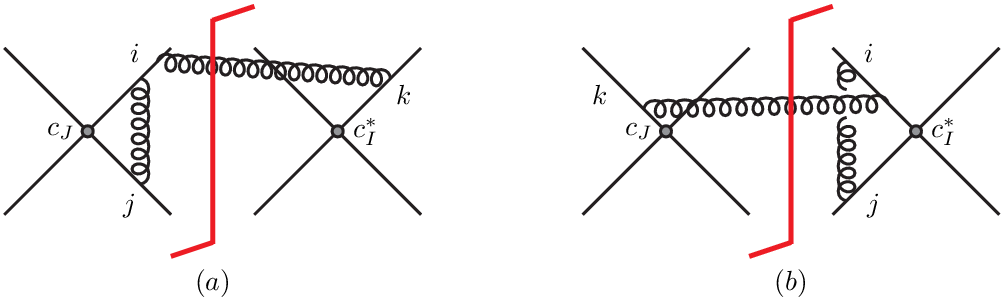
\includegraphics[width=0.7\textwidth]{plots/diagram4-pecjak.png}
  \end{center}
  \caption{
    Three-Wilson-line, mixed real-virtual integrals, which add up to scaleless
    integral.
  }
  \label{fig:pecjak4}
\end{figure}
%

The single-gluon cut integrals of Fig.~\ref{fig:pecjak4} read
%
\begin{eqnarray}
  \bar{I}_{8, ijk}^{(a)} &= &
  n_i \cdot n_j\; n_i \cdot n_k\; 
  \int d^d k\, d^d l\; 
  \frac{\delta_+(k^2) \,
    \; \delta^{(2)}(q_\perp-k_\perp)}
    {(n \cdot k)^\alpha\; (n \cdot l)^\beta \; 
    n_i \cdot k \; n_i \cdot (k+l) \; n_j \cdot l \; n_k \cdot k} \,,
  \\
  \bar{I}_{8, ijk}^{(b)} &= &
  n_i \cdot n_j\; n_i \cdot n_k\; 
  \int d^d k\, d^d l\; 
  \frac{\delta_+(k^2) \,
    \; \delta^{(2)}(q_\perp-k_\perp)}
    {(n \cdot k)^\alpha\; (n \cdot l)^\beta \; 
    n_i \cdot l \; n_i \cdot (k+l) \; n_j \cdot l \; n_k \cdot k} \,.
  %\label{eq:}
\end{eqnarray}
%
This type of diagrams are scaleless and vanish in the fully massless case
discussed in~\cite{Ferroglia:2012uy} but they do not need to vanish here as in
our case two outgoing legs are massive. 

\section{Vacuum polarization integrals}
%-----------------------------------------------------------------------------
\subsubsection{Direct calculation}

After a little bit of calculation, we get
%
\begin{equation}
  2\im\, \calM_{g\to g} =  
  2 g^2 T_R \int\frac{d^4 k}{(2\pi)^2}
  \frac{\delta_+(k^2)\, \delta_+((p-k)^2)}{k_+^\alpha\, (p-k)_+^\alpha}
  \left[
    2k^\mu p^\nu + 2p^\mu k^\nu - 4 k^\mu k^\nu - p^2 g^{\mu\nu}
  \right]\,.
  %\label{eq:}
\end{equation}
% 
The above can be written in general as a tensor
%
\begin{equation}
  \Pi^{\mu\nu} = {\cal N} (p^2, \alpha)\, 
  T^{\mu\nu} (p^\mu,p^\nu, n^\mu, n^\nu, g^{\mu\nu})\,,
  %\label{eq:}
\end{equation}
%
where the form of $T^{\mu\nu}$ can be determined by considering all possible
combinations of external vectors, whereas the normalization, $\calN $, has to be
calculated directly. The corresponding integral, after a series of
transformations, reduces to 
%
\begin{equation}
  \calN = 
  \int_0^1 d x\, x^{-\alpha}\int_{-\pi}^\pi d\theta
  \left(1-2\pbar \sqrt{x \xbar}\cos\theta\right)^{2\alpha-2}
  \left(K_0(1-2\pbar \sqrt{x \xbar}\cos\theta)-x\right)^{-\alpha}\,,
  %\label{eq:}
\end{equation}
%
where
\begin{align}
  \xbar &= 1 - x\,, \\[0.5em]
  \pbar &= \frac{p_T}{p_+ p_-}\,, \\[0.5em]
  K_0   &= \frac{p_+ p_-}{p^2}\,.
\end{align}



%-----------------------------------------------------------------------------
\bibliographystyle{unsrt}
\bibliography{precision-qcd}

\end{document}
